\chapter{IPv6: Part 3}\label{ipv6-part-3}

\section{Correction to Prior
Lectures}\label{correction-to-prior-lectures}

RFC Requirements for IPv6 Address Representation

\begin{itemize}
\tightlist
\item
  Leading 0s MUST be removed

  \begin{itemize}
  \tightlist
  \item
    This - 2001 : 0db8 : 0000 : 0001 : 0f2a : 4fff : fea3 : 00b1
  \item
    Becomes - 2001 : db8 : 0 : 1 : f2a : 4fff : fea3 : b1
  \end{itemize}
\item
  :: MUST be used to shorten the longest string of all-0 quartets

  \begin{itemize}
  \tightlist
  \item
    If there is only ONE all-0 quartet, don't use `::'
  \item
    This - 2001 : 0000 : 0000 : 0000 : 0f2a : 0000 : 0000 : 00b1
  \item
    Becomes - 2001 :: f2a : 0 : 0 : b1
  \end{itemize}
\item
  If there are two equal-length choices for the :: , use :: to the
  shorten the one on the LEFT

  \begin{itemize}
  \tightlist
  \item
    This - 2001 : 0db8 : 0000 : 0000 : 0f2a : 0000 : 0000 : 00b1
  \item
    Becomes - 2001 : db8 :: f2a : 0 : 0 : b1
  \end{itemize}
\item
  Hexadecimal characters `a', `b', `c', `d', `e', and `f' MUST be
  written using lower-case, NOT upper case A B C D E F
\end{itemize}

IPv6 HEADER

\begin{figure}
\centering
\pandocbounded{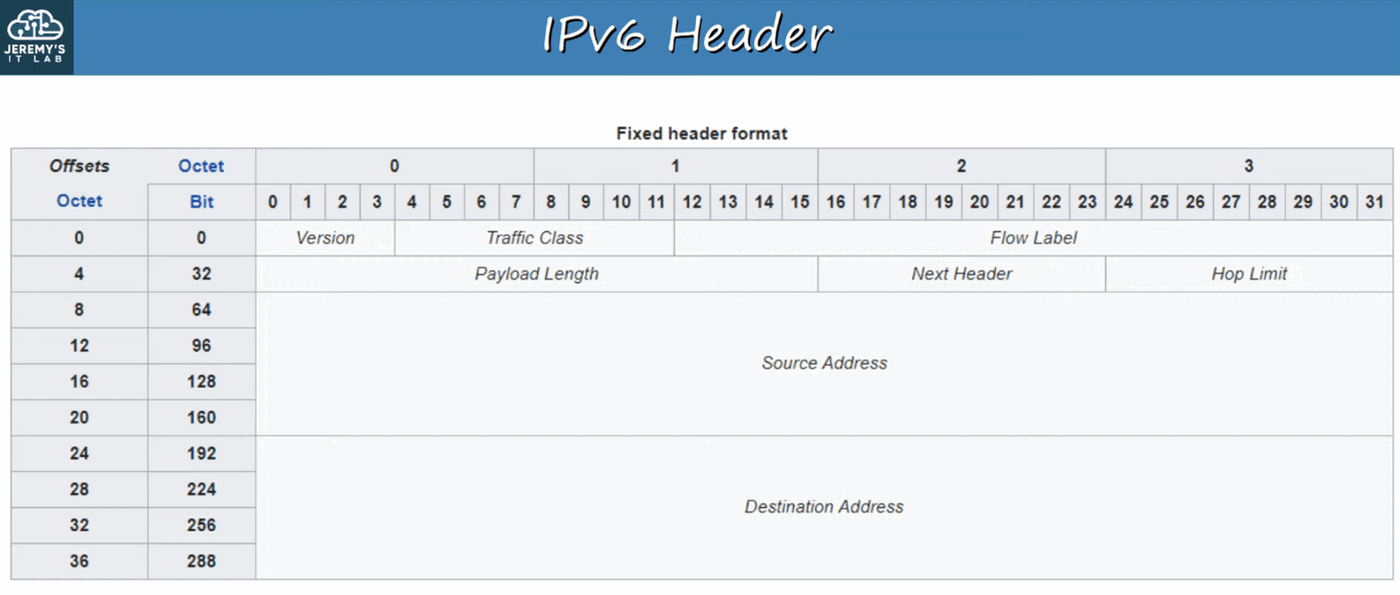
\includegraphics[keepaspectratio,alt={image}]{images/34-ipv6-part3/img-001.png}}
\end{figure}

Length is ALWAYS 40 bytes (Fixed Header)

Version (4 bits)

\begin{itemize}
\tightlist
\item
  Indicates version of IP used
\item
  Fixed value of `6' (0b0110) to indicate IPv6
\end{itemize}

Traffic Class (8 bits)

\begin{itemize}
\tightlist
\item
  Used for QoS (Quality of Service) to indicate high-priority traffic
\item
  Example: IP phone traffic, live video calls, etc.
\end{itemize}

Flow Label (20 bits)

\begin{itemize}
\tightlist
\item
  Identifies specific traffic ``flows'' (communication between Source
  and Destination)
\end{itemize}

Payload Length (16 bits)

\begin{itemize}
\tightlist
\item
  Indicates the LENGTH of the PAYLOAD (the encapsulation LAYER 4
  SEGMENT) \textbf{in bytes}
\item
  The length of the IPv6 header, itself, isn't included, because it's
  ALWAYS 40 bytes
\end{itemize}

Next Header (8 bits)

\begin{itemize}
\tightlist
\item
  Indicates the TYPE of the `next header' (header of the encapsulated
  SEGMENT)

  \begin{itemize}
  \tightlist
  \item
    Example: TCP or UDP
  \end{itemize}
\item
  Same function as the IPv4 header's `Protocol' field
\end{itemize}

Hop Limit (8 bits)

\begin{itemize}
\tightlist
\item
  Value in this field decrements by 1 every time a ROUTER forwards it.
  If it reaches `0', the PACKET is discarded (similar to IPv4 TTL field
  )
\end{itemize}

Source Address (128 bits)

\begin{itemize}
\tightlist
\item
  Packet's SOURCE address
\end{itemize}

Destination Address (128 bits)

\begin{itemize}
\tightlist
\item
  Packet's DESTINATION address
\end{itemize}

\section{Solicited-Node Multicast
Address}\label{solicited-node-multicast-address}

\begin{itemize}
\tightlist
\item
  An IPv6 SOLICITED-NODE Multicast Address is calculated from a UNICAST
  ADDRESS
\end{itemize}

How to generate a SOLICITED-NODE Multicast Address

\begin{figure}
\centering
\pandocbounded{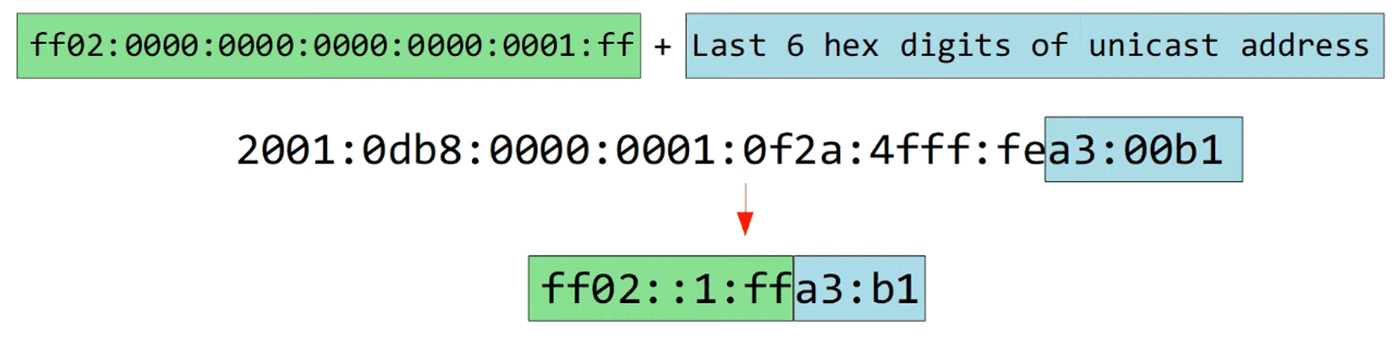
\includegraphics[keepaspectratio,alt={image}]{images/34-ipv6-part3/img-002.png}}
\end{figure}

Note the automatically joined group addresses for this IPv6 Interface

\begin{figure}
\centering
\pandocbounded{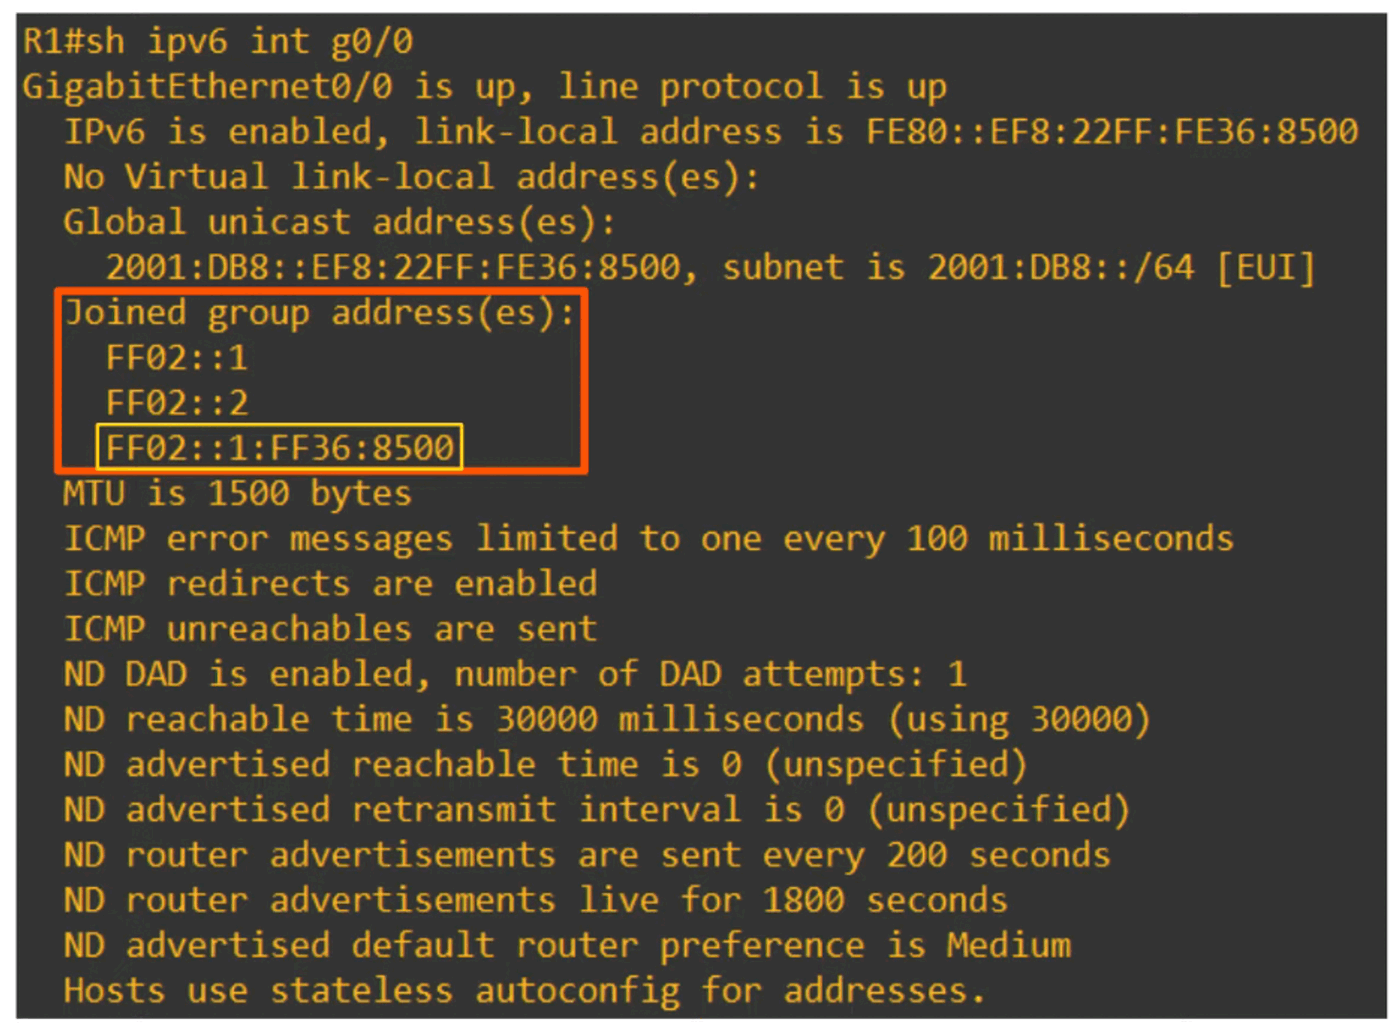
\includegraphics[keepaspectratio,alt={image}]{images/34-ipv6-part3/img-003.png}}
\end{figure}

\section{Neighbor Discovery Protocol
(NDP)}\label{neighbor-discovery-protocol-ndp}

\begin{itemize}
\item
  NEIGHBOR DISCOVERY PROTOCOL (NDP) is a PROTOCOL used with IPv6
\item
  It has various functions and one of those functions is to replace ARP,
  which is no longer used in IPv6
\item
  The ARP-like function of NDP uses ICMPv6 and SOLICITED-MODE Multicast
  Addresses to learn the MAC ADDRESS of other HOSTS (ARP in IPv4 uses
  Broadcast Messages)
\item
  TWO MESSAGES types are used:

  \begin{itemize}
  \item
    \begin{enumerate}
    \def\labelenumi{\arabic{enumi})}
    \tightlist
    \item
      NEIGHBOR SOLICITATION (NS)
    \end{enumerate}

    \begin{itemize}
    \tightlist
    \item
      ICMPv6 Type 135
    \end{itemize}
  \item
    2) NEIGHBOR ADVERTISEMENT (NA)

    \begin{itemize}
    \tightlist
    \item
      ICMPv6 Type 136
    \end{itemize}
  \end{itemize}
\end{itemize}

\begin{figure}
\centering
\pandocbounded{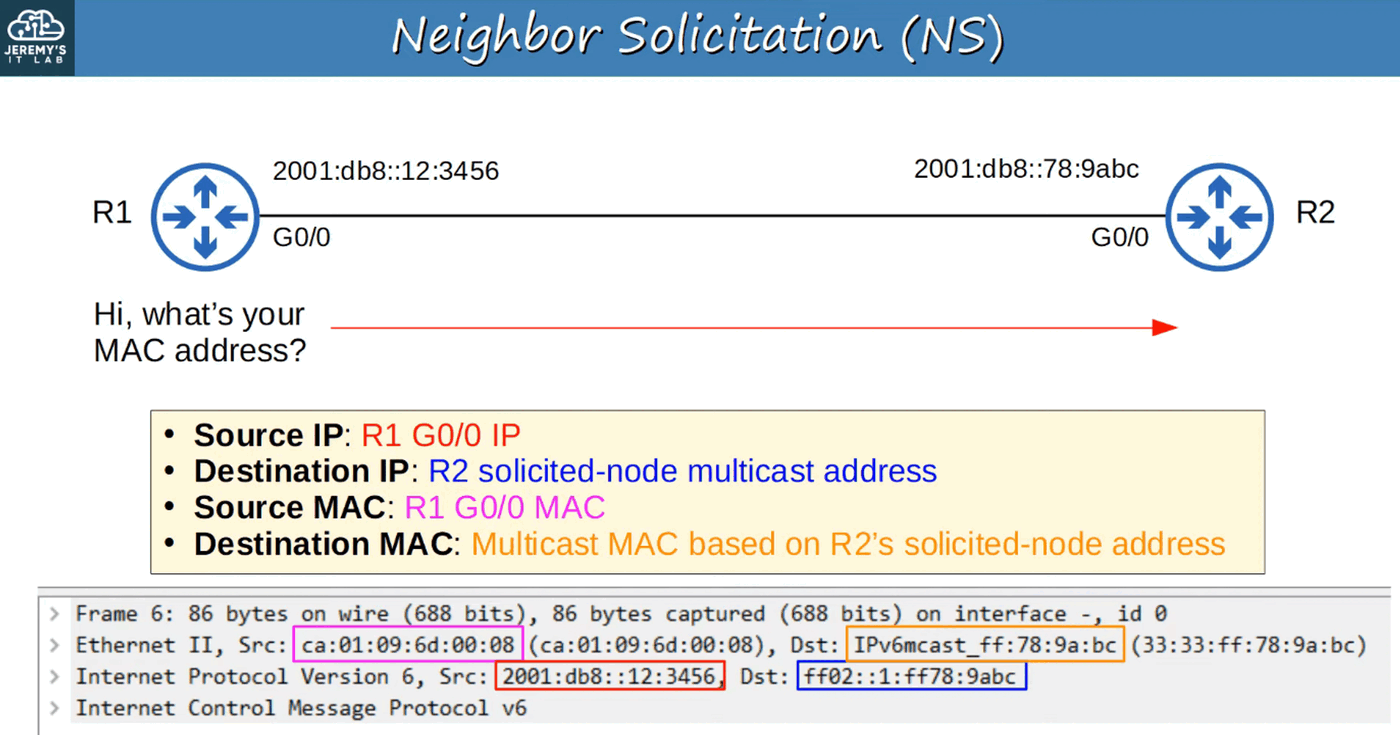
\includegraphics[keepaspectratio,alt={image}]{images/34-ipv6-part3/img-004.png}}
\end{figure}

\begin{figure}
\centering
\pandocbounded{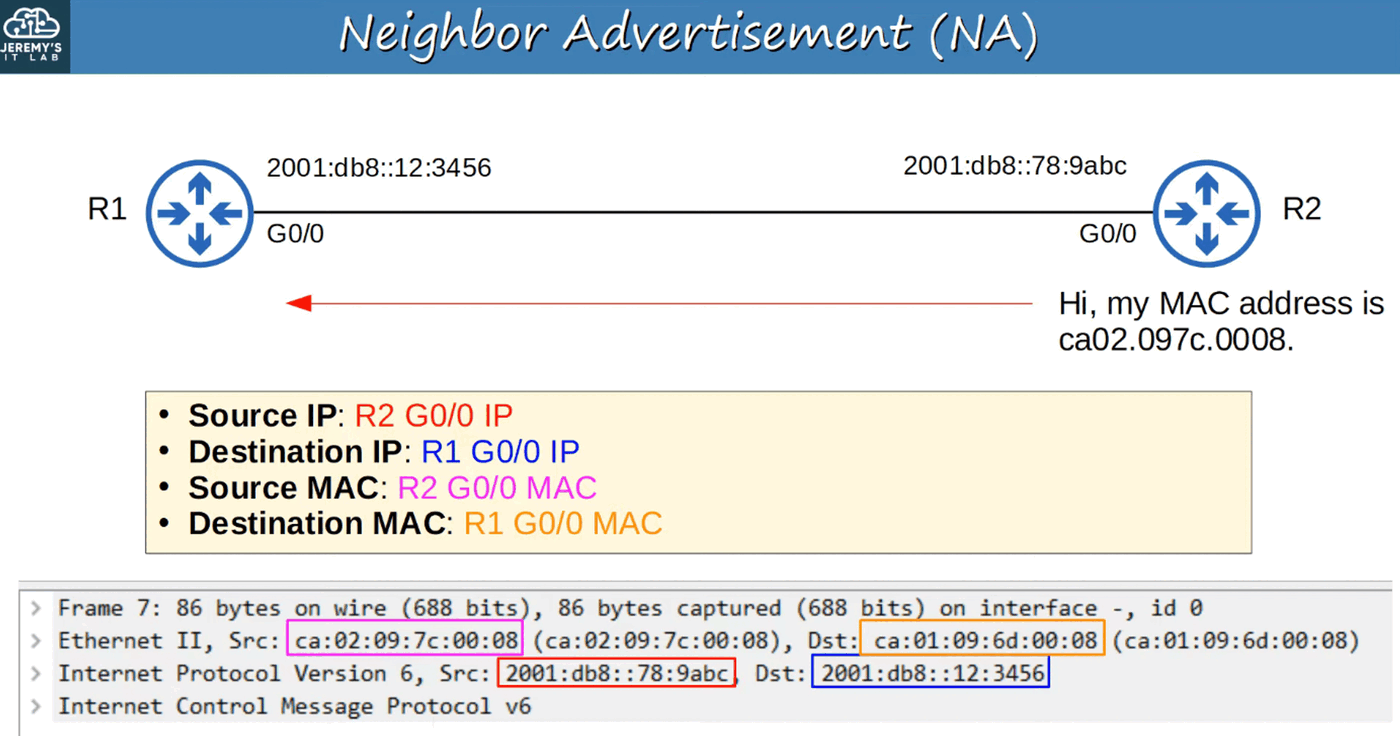
\includegraphics[keepaspectratio,alt={image}]{images/34-ipv6-part3/img-005.png}}
\end{figure}

IPv6 NEIGHBOR TABLE

\begin{figure}
\centering
\pandocbounded{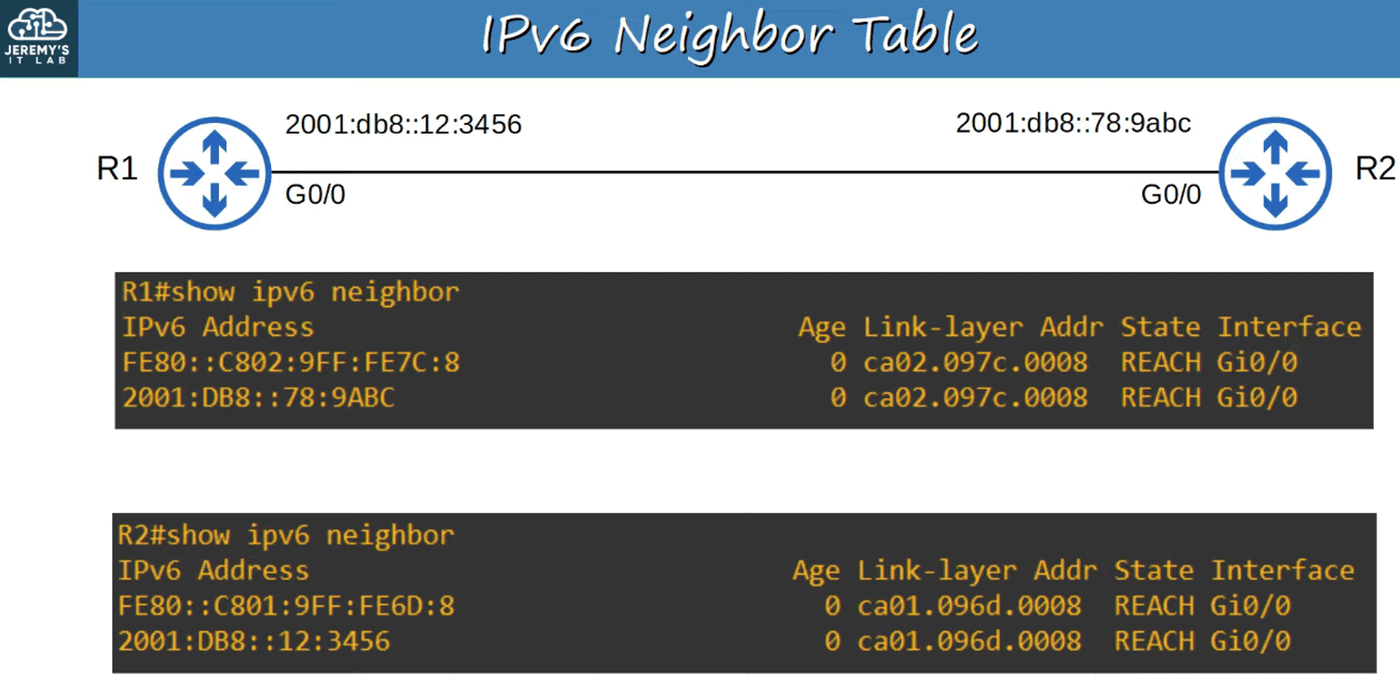
\includegraphics[keepaspectratio,alt={image}]{images/34-ipv6-part3/img-006.png}}
\end{figure}

\begin{itemize}
\item
  Another function of NDP allows HOSTS to automatically discover ROUTERS
  on the LOCAL NETWORK
\item
  TWO MESSAGES are used for this process:

  \begin{itemize}
  \tightlist
  \item
    ROUTER SOLICITATION (RS)

    \begin{itemize}
    \tightlist
    \item
      ICMPv6 Type 133
    \item
      Sent to Multicast Address \passthrough{\lstinline!FF02::2!} (All
      Routers)
    \item
      Asks ALL ROUTERS on the Local Link to identify themselves
    \item
      Sent when an INTERFACE is enabled / HOST is connected to the
      NETWORK
    \end{itemize}
  \item
    ROUTER ADVERTISEMENT (RA)

    \begin{itemize}
    \tightlist
    \item
      ICMPv6 Type 134
    \item
      Sent to Multicast Address \passthrough{\lstinline!FF02::1!} (All
      Nodes)
    \item
      The ROUTER announces its presence, as well as other information
      about the link
    \item
      These messages are sent in response to RS messages
    \item
      They are also sent periodically, even if the ROUTER hasn't
      received an RS
    \end{itemize}
  \end{itemize}
\end{itemize}

\begin{figure}
\centering
\pandocbounded{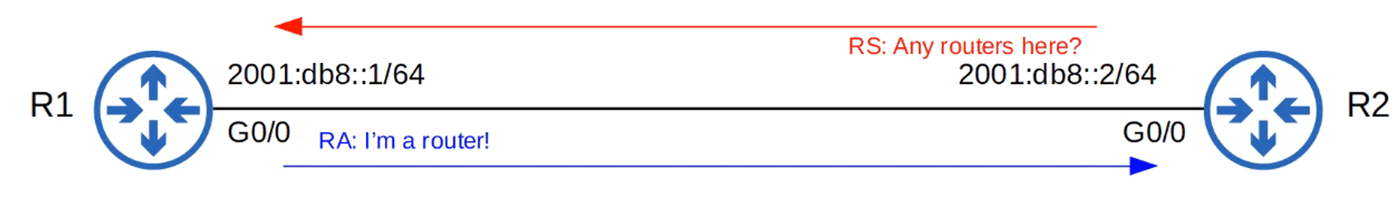
\includegraphics[keepaspectratio,alt={image}]{images/34-ipv6-part3/img-007.png}}
\end{figure}

\section{SLAAC}\label{slaac}

\begin{itemize}
\tightlist
\item
  Stands for \textbf{STATELESS ADDRESS AUTO-CONFIGURATION}
\item
  HOSTS use the RS / RA messages to learn the IPv6 Prefix of the LOCAL
  LINK (ie: 2000:db8:: /64) and then automatically generate an IPv6
  Address
\item
  Using the
  \passthrough{\lstinline!ipv6 address prefix / prefix-length eui-64!}
  command, you need to manually enter the prefix
\item
  Using the \passthrough{\lstinline!ipv6 address autoconfig!} command,
  you DON'T need to enter the prefix. The device uses NDP to learn the
  prefix used on the local link
\item
  The device will use EUI-64 to generate the INTERFACE ID or it will be
  randomly generated (depending on the device / maker)
\end{itemize}

\begin{figure}
\centering
\pandocbounded{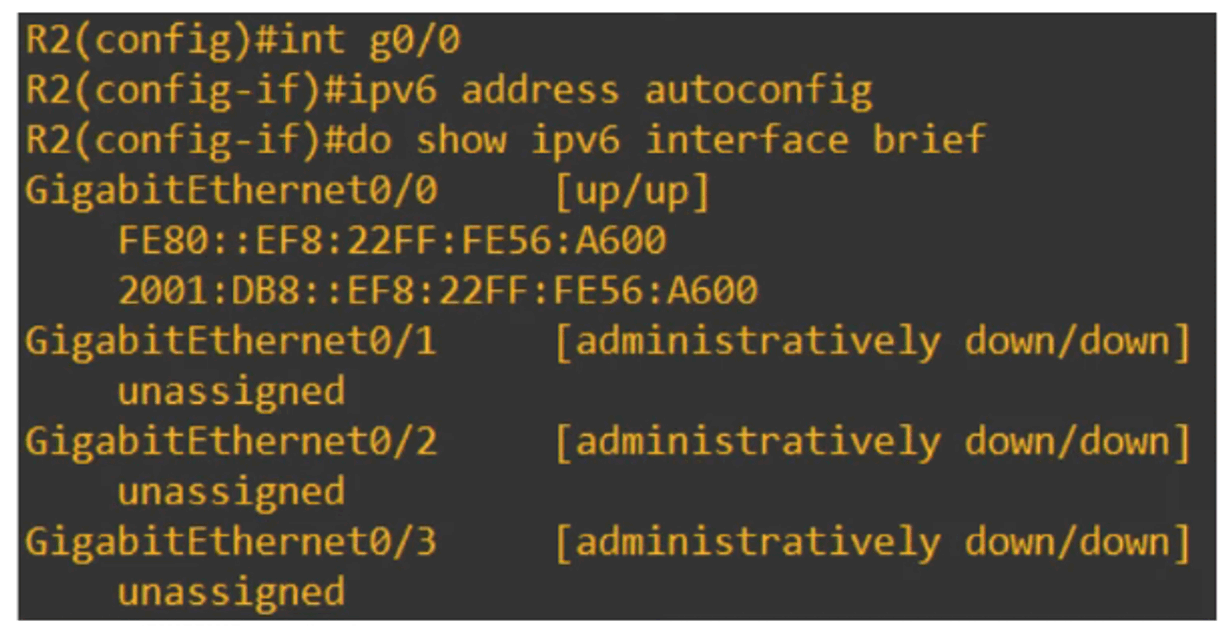
\includegraphics[keepaspectratio,alt={image}]{images/34-ipv6-part3/img-008.png}}
\end{figure}

\section{Duplicate Address Detection
(DAD)}\label{duplicate-address-detection-dad}

\begin{itemize}
\tightlist
\item
  One final point about NDP!
\item
  Duplicate Address Detection (DAD) allows HOSTS to check if other
  devices on the Local Link are using the same IPv6 Address
\item
  Any time an IPv6-enabled interface initializes
  (\passthrough{\lstinline!no shutdown!} command) or an IPv6 ADDRESS is
  configured on an INTERFACE (by any method: manual, SLAAC, etc.) it
  performs DAD
\item
  DAD uses TWO MESSAGES you learned earlier : NS and NA
\item
  The HOST will send an NS to its own IPv6 ADDRESS.

  \begin{itemize}
  \tightlist
  \item
    If it doesn't get a reply, it KNOWS the ADDRESS is unique
  \item
    If it DOES get a reply, it means ANOTHER HOST on the NETWORK is
    already using that ADDRESS
  \end{itemize}
\end{itemize}

IPv6 STATIC ROUTING

\begin{itemize}
\tightlist
\item
  IPv6 ROUTING works the same as IPv4 ROUTING
\item
  However, the TWO processes are separate on the ROUTER, and the TWO
  routing tables are separate, as well.
\item
  IPv4 ROUTING is enabled BY DEFAULT
\item
  IPv6 ROUTING is disabled BY DEFAULT

  \begin{itemize}
  \tightlist
  \item
    MUST BE ENABLED with the
    \passthrough{\lstinline!ipv6 unicast-routing!} command
  \end{itemize}
\item
  If IPv6 ROUTING is disabled, the ROUTER will be able to SEND and
  RECEIVE IPv6 traffic, but will not \emph{route} IPv6 traffic (ie: will
  NOT FORWARD it between NETWORKS)
\end{itemize}

\begin{figure}
\centering
\pandocbounded{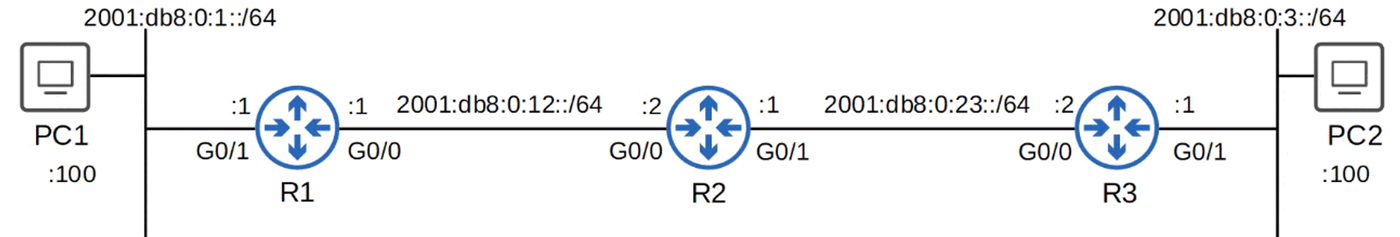
\includegraphics[keepaspectratio,alt={image}]{images/34-ipv6-part3/img-009.png}}
\end{figure}

\begin{figure}
\centering
\pandocbounded{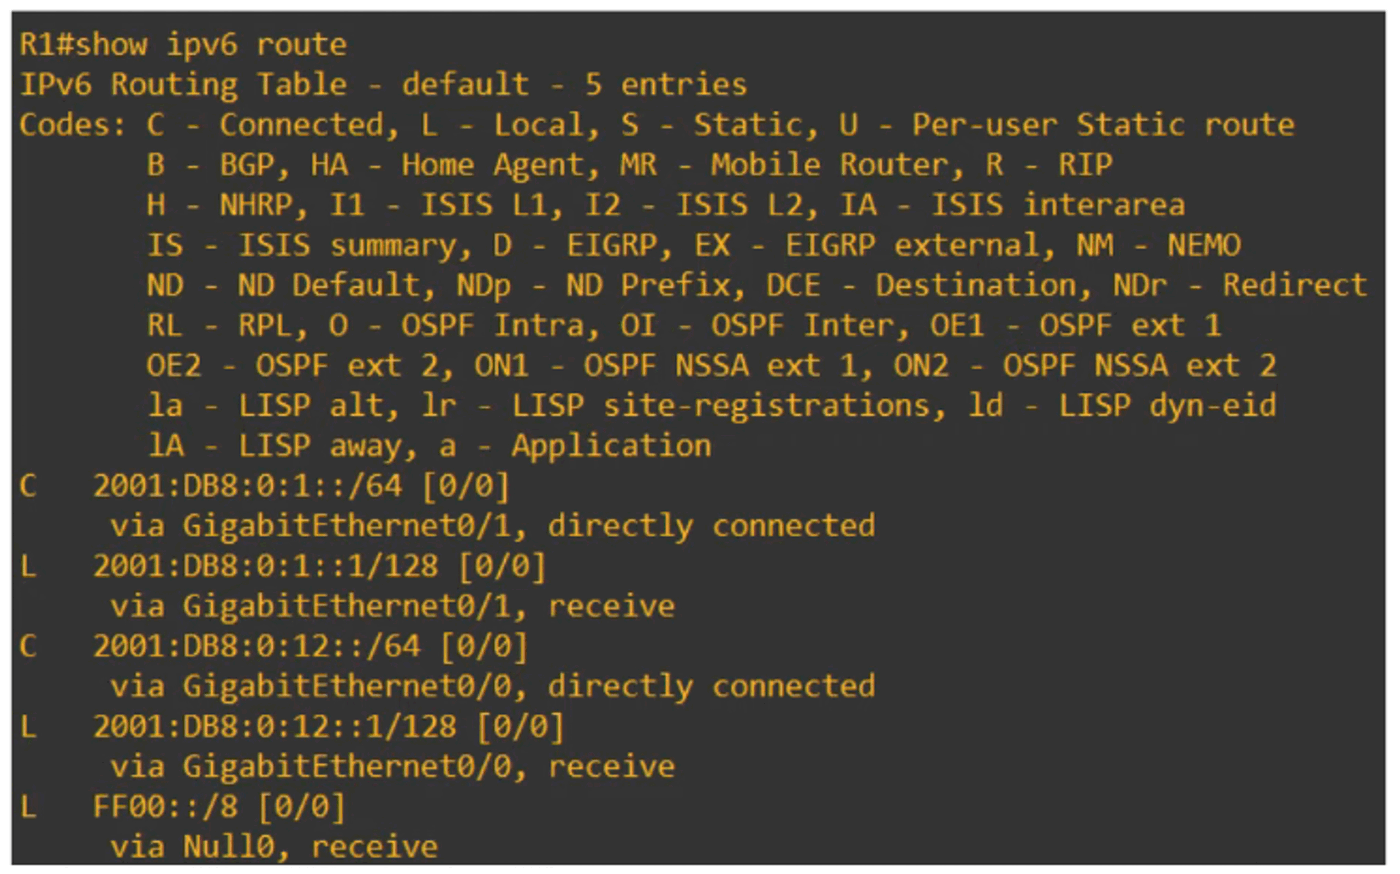
\includegraphics[keepaspectratio,alt={image}]{images/34-ipv6-part3/img-010.png}}
\end{figure}

\begin{itemize}
\tightlist
\item
  A CONNECTED NETWORK ROUTE is automatically added for EACH CONNECTED
  NETWORK
\item
  A LOCAL HOST ROUTE is automatically added for each ADDRESS configured
  on the ROUTER
\item
  Routes for Link-Local ADDRESSES are not added to the ROUTING TABLE
\end{itemize}

\begin{figure}
\centering
\pandocbounded{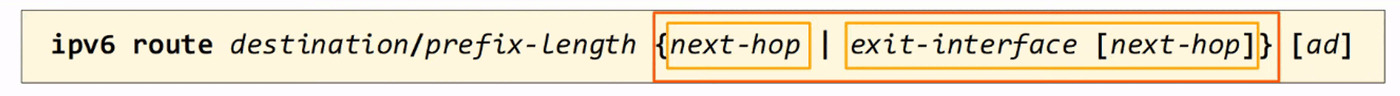
\includegraphics[keepaspectratio,alt={image}]{images/34-ipv6-part3/img-011.png}}
\end{figure}

Everything is configured similar to normal static routes in IPv4

{[}AD{]} = Administrative Distance. You NEED this value in order to
configure a STATIC ROUTE

DIRECTLY ATTACHED Static Route:

\begin{itemize}
\tightlist
\item
  Only the EXIT INTERFACE is specified
\item
  \passthrough{\lstinline!ipv6 route destination / prefix-length exit-interface!}
\item
  Example :
  \passthrough{\lstinline!\~\~R1(config)\# ipv6 route 2001:db8:0:3:: /64 g0/0\~\~!}
\end{itemize}

\begin{tipbox}

In IPv6, you CANNOT use DIRECTLY ATTACHED Static Routes if the INTERFACE
is an ETHERNET INTERFACE

\end{tipbox}

RECURSIVE Static Route:

\begin{itemize}
\tightlist
\item
  Only the Next-Hop is specified
\item
  \passthrough{\lstinline!ipv6 route destination / prefix-length next-hop!}
\item
  Example:
  \passthrough{\lstinline!R1(config)\# ipv6 route 2001:db8:0:3::/64 2001:db8:0:12::2!}
\end{itemize}

FULLY SPECIFIED Static Route:

\begin{itemize}
\tightlist
\item
  Both the Exit Interface and Next Hop are specified
\item
  \passthrough{\lstinline!ipv6 route destination / prefix-length exit-interface next-hop!}
\item
  Example:
  \passthrough{\lstinline!R1(config)\# ipv6 route 2001:db8:0:3::/64 g0/0 2001:db8:0:12::2!}
\end{itemize}

(NOTE THAT THESE ROUTES ARE ALL RECURSIVE : They specify the Next-Hop)

\section{Network Route}\label{network-route}

\passthrough{\lstinline!R1(config)\# ipv6 route 2001:db8:0::/64 2001:db8:0:12::2!}

This is a route to R3/PC2 NETWORK via R2's G0/0 INTERFACE

(We did this in Day 32's Lab)

\section{Host Route}\label{host-route}

\passthrough{\lstinline!R2(config)\# ipv6 route 2001:db8:0:1::100/128 2001:db8:0:12::1!}

\passthrough{\lstinline!R2(config)\# ipv6 route 2001:db8:0:3::100/128 2001:db8:0:23::2!}

This is a route from R2 to PC1 and PC2 using the ``next hop'' ADDRESSES
of R1 and R3 G0/0 INTERFACES

Note the /128 prefix. This is how SPECIFIC IPv6 ADDRESSES are written

\section{Default Route}\label{default-route}

\passthrough{\lstinline!R3(config)\# ipv6 route ::/0 2001:db8:0:23::1!}

::/0 is the IPv6 equivalent of 0.0.0.0/0 in IPv4

\section{Floating Static Routes}\label{floating-static-routes}

\begin{itemize}
\tightlist
\item
  Require you to increase the {[}AD{]} number HIGHER than the currently
  used NETWORK IGP AD value
\end{itemize}

\section{Link-Local Next Hops}\label{link-local-next-hops}

\begin{figure}
\centering
\pandocbounded{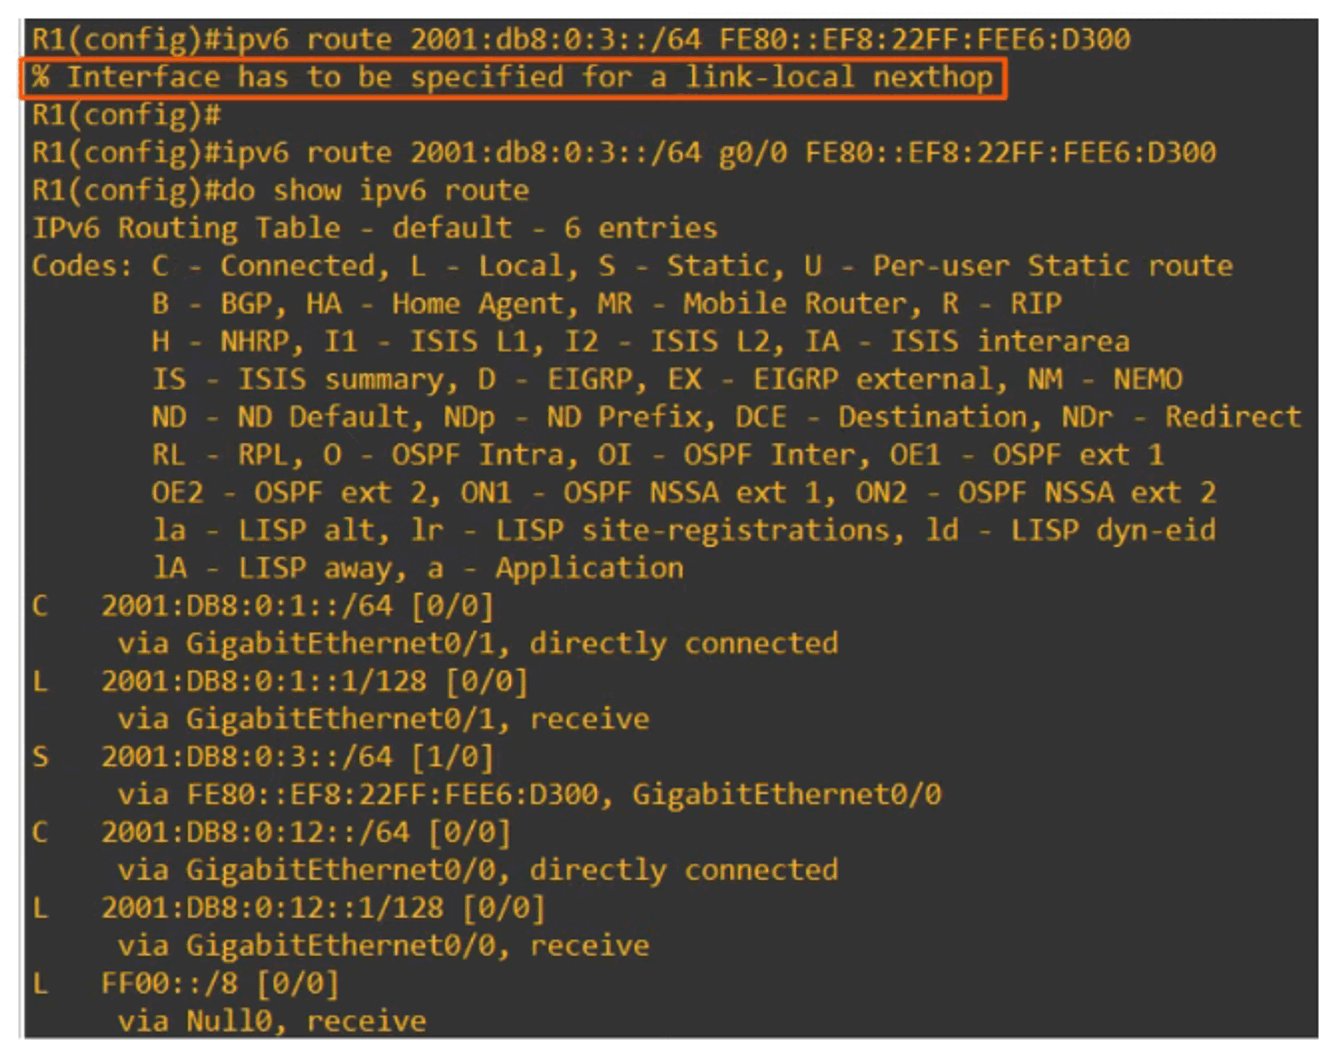
\includegraphics[keepaspectratio,alt={image}]{images/34-ipv6-part3/img-012.png}}
\end{figure}

You HAVE to specify the INTERFACE name when using Link-Local Next-Hops

This is EXACTLY like a FULLY-SPECIFIED STATIC ROUTE
